\documentclass[12pt, a4paper]{report}
\usepackage[utf8]{inputenc}
\usepackage[IL2]{fontenc}
\usepackage[czech]{babel}
\usepackage{graphicx}
\usepackage{epstopdf}
\usepackage{url}

\begin{document}
	\begin{titlepage}
	
\includegraphics[width=5cm,natwidth=601,natheight=314]{obrazky/logo.png}
		
	\vspace{4cm}
		\begin {center}
		{\Huge SEMESTRÁLNÍ PRÁCE\\ Z~PŘEDMĚTU KIV/ZVI\\}
		\vspace{1cm}
		{\huge Analýza sekvence mikroskopických snímků, segmentace, detekce objektů\\}
		\end {center}
	\vspace{6cm}
			
	\noindent vypracovali: Denisa Tarantíková, Radek Vais \\
				studijní čísla: A13B0445P, A13B0457P\\
				email:	denitara@students.zcu.cz, vaisr@students.zcu.cz\\
				datum:	15. 6. 2016
	\end{titlepage}

\tableofcontents
\chapter{Úvod}
	Cílem této semestrální práce bude analyzovat sekvenci mikroskopických snímků a detekovat v~nich jevy zvané inkluze. Data, která budou použita pro vývoj aplikace, byla snímána infračerveným mikroskopem se zvětšením 5$\times$ (1.09 $\mu$m/px) a krokem mezi řezy (snímky) 0.2 $\mu$m, snímaným materiálem byla směs kadmia a teluru. 
	
	Inkluze jsou defekty vznikající při tuhnutí taveniny na místech, kde je více atomů teluru/kadmia, než by bylo v~pevné fázi za dané teploty. Z~hlediska energie je výhodnější na těchto místech vytvořit kapalné shluky obohacené o jednu z~komponent. Během tuhnutí povrch defektu zmenšuje svůj objem a přebytečná komponenta vytvoří ve středu defektu koncentrované \uv{kapky}.\footnote{	Zdroj: ŠEDIVÝ, L.: \emph{Difúze přirozených defektů a příměsí v CdTe/CdZnTe.} Praha: Univerzita Karlova v Praze, Matematicko-fyzikální fakulta, 2012. 84 s. Vedoucí diplomové práce Doc. Ing. Eduard Belas, CSc.} Tento jev se může vyskytovat i v~jiných materiálech. 

Výstupem práce bude kromě aplikace pro detekci inkluzí napsané v~jazyce C++ i soubor ve formátu *.xml, ve kterém budou uvedeny souřadnice inkluzí ve snímku a názvy snímků, na kterých se vyskytují.
\chapter{Zadání}
Obecné pokyny a pravidla pro vypracování semestrální práce:
\begin{enumerate}
	\item Součástí semestrální práce je teoretické řešení zadaného úkolu a programová realizace, která může být napsána v libovolném vhodném programovacím jazyku. Programová realizace by měla obsahovat základní funkce:
	\begin{itemize}
		\item{výběr souboru vstupního snímku [formát *.BMP, *.JPG,…] a jeho zobrazení}
		\item{zobrazování dílčích snímků jako výstupů jednotlivých fází zpracování úlohy včetně výsledku konečného}
		\item{volba pořadí jednotlivých metod předzpracování (pokud bude typ zadané úlohy vyžadovat
předzpracování) a vlastního zpracování úlohy dle zadání}
		\item{navržené algoritmy budou optimalizovány podle časového kritéria}
		\item{funkce "Krok zpět", minimálně o 1 krok (podle charakteru úlohy)}
		\item{uložení výsledného snímku do výstupního obrazového souboru, formát viz vstupní snímek}
		\item{uložení výsledných hodnot do výstupních souborů v předepsaném a komentovaném formátu,
např. tabulky hodnot, příznakové vektory,…}
	\end{itemize}
\item{Pokud to zadané téma vyžaduje, bude součástí programové realizace také soubor metod pro
zobrazení globálních charakteristik a předzpracování snímků.}		
\item{Součástí odevzdané práce bude vypracovaný referát, použité testovací snímky (zadané nebo
vlastní), programová realizace úlohy ve spustitelné verzi, tj. *.exe, včetně všech potřebných
knihoven a zdrojových souborů programu + prezentace v PowerPointu.}
\item{Semestrální práce bude obsahovat rozbor dosažených výsledků, tzn. zhodnocení jednotlivých
aplikovaných metod, popis jejich pozitivních a negativních vlastností, porovnání výsledků podle
vlastností použitých snímků, srovnání funkce jednotlivých algoritmů, resp. výsledků
a mezivýsledků, s dostupným programovým produktem, např. CVIP Tools,…}
\end{enumerate}
\chapter{Analýza úlohy}
	\section{Předzpracování}
	Původní snímek (na obrázku 3.1) bude nutné nejdříve převést na šedotónový kvůli barevnému měřítku v~pravé dolní části. Tmavé objekty hvězdicovitého až kulatého tvaru jsou potenciálními inkluzemi (na obrázku 3.2 lze vidět snímek inkluze ve 20násobném zvětšení). Dále lze na snímku pozorovat různé typy šumu: vlny způsobené strukturou materiálu, prach, škrábance, otisky prstů apod. Tyto šumy bude třeba co nejvíce potlačit, aby bylo možné inkluze lépe detekovat.
		
	\begin{figure}[!htb]
	\centering
	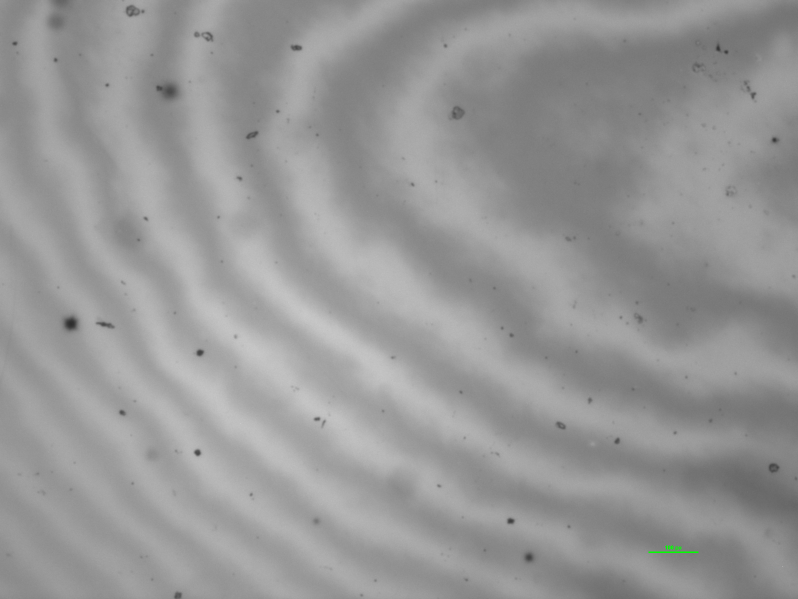
\includegraphics[scale=0.4]{obrazky/puvodni.png}
	\label{fig:puvodni}
	\caption{Původní snímek}
	\end{figure}
	
	\begin{figure}[!htb]
	\centering
	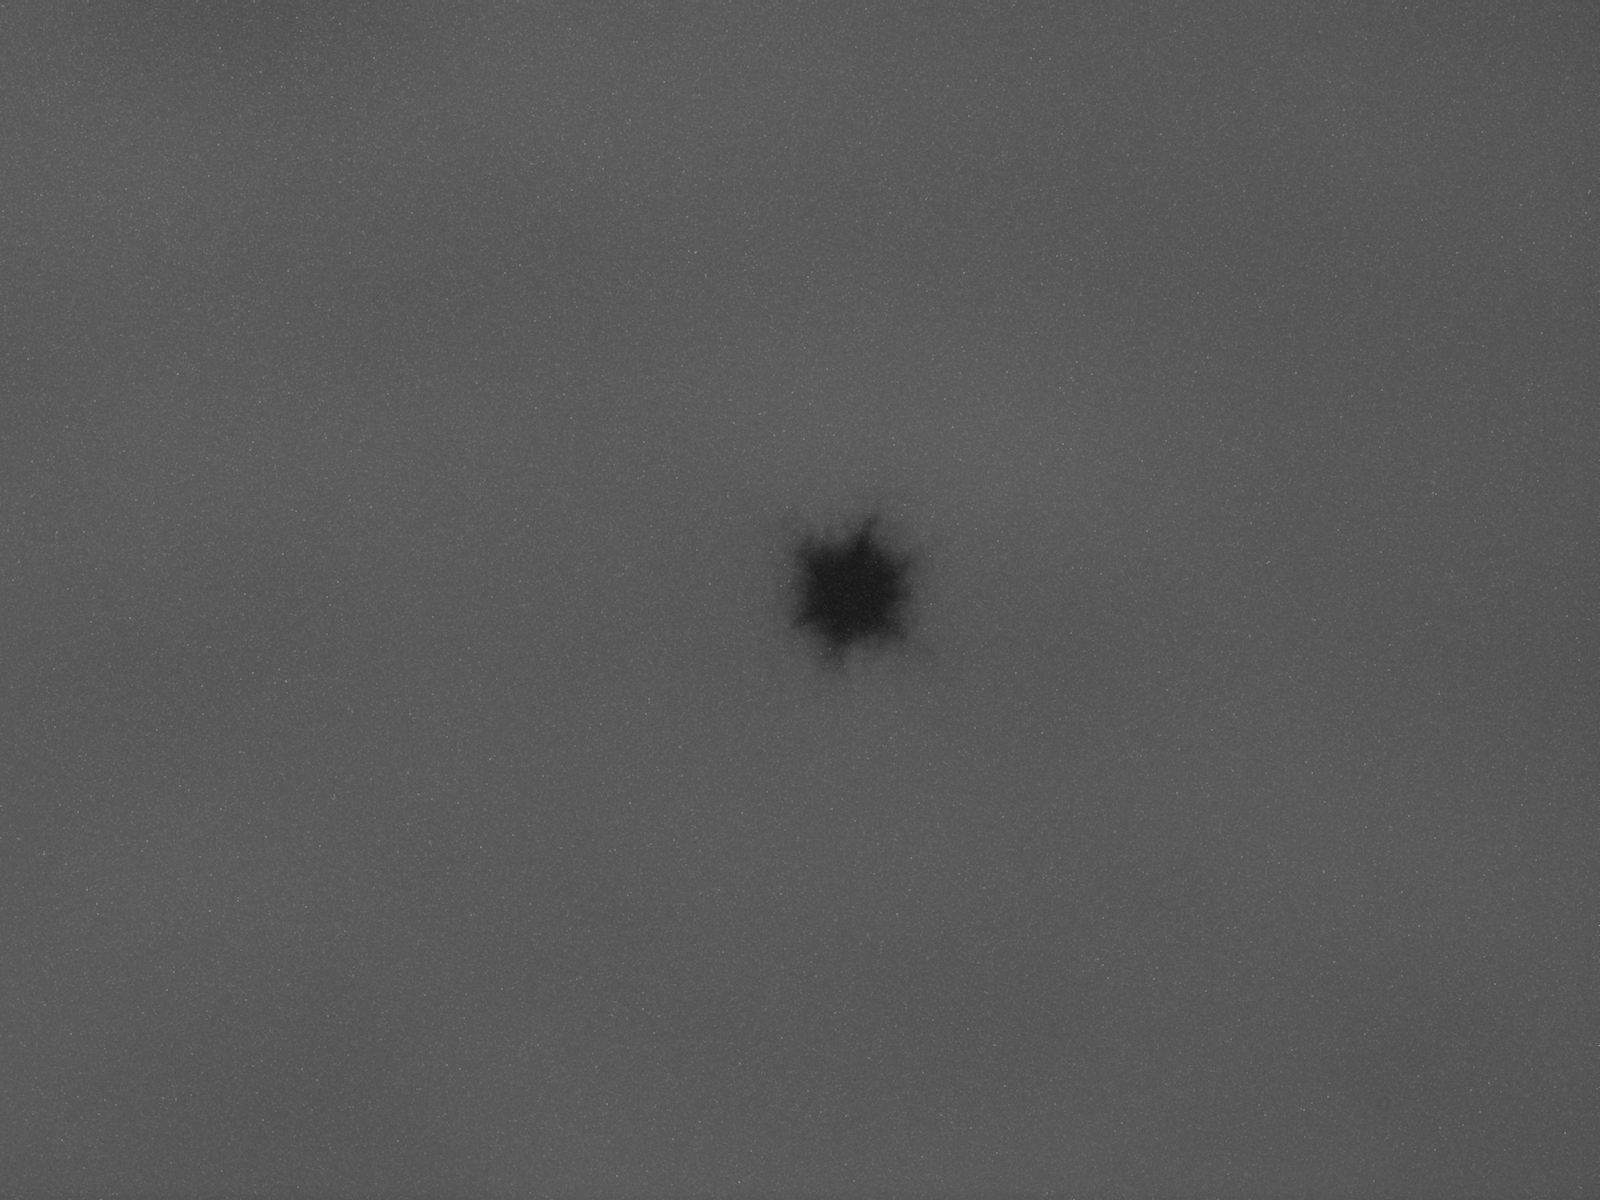
\includegraphics[scale=0.12]{obrazky/konvoluce.png}
	\label{fig:inkluze}
	\caption{Inkluze}
	\end{figure}	

	Dle histogramu původního snímku na obrázku 3.3 si lze povšimnout, že většina obrazových bodů na stupnici jasu od 0 do 255 nabývá hodnot v~intervalu přibližně od 100 do 200. Budeme uvažovat, že v~ostatních snímcích v~zadané sekvenci je přibližně stejné rozložení hodnot jasu. Vzhledem k~tomu, že inkluze se jeví tmavé v~porovnání s~ostatními obrazovými body snímku, zvýrazněním tmavých odstínů oproti světlým bychom docílili \uv{vystoupení} inkluzí. Pro dosažení tohoto výsledku přebarvíme hodnoty vysokých jasů tak, že jasy vyšší než zvolená mezní hodnota $M$ (včetně) nabudou nejvyššího jasu (255). Tím potlačíme šum, jehož jas nabývá vysokých hodnot (např. vlny). Zbylé hodnoty \uv{roztáhneme} po celém intervalu 0 až 255 vynásobením koeficientem $\frac{256}{M}$, kde v~čitateli je počet hodnot v~celém intervalu a ve jmenovateli počet zbylých (\uv{nesjednocovaných}) hodnot. Touto operací zvýšíme kontrast, a tak usnadníme kontrolu výskytu inkluzí lidským okem. 
	
	\begin{figure}[!htb]
	\centering
	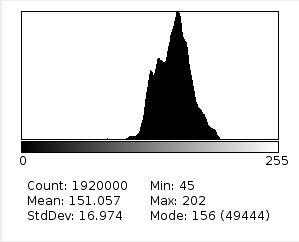
\includegraphics[scale=0.65]{obrazky/puvodni_histogram.png}
	\label{fig:puvodni_histogram}
	\caption{Histogram původního snímku}
	\end{figure}	
	
	Hodnotu, kterou zvolíme jako mezní, určíme na intervalu od 100 do 150 (150 je vrchol histogramu na obrázku 3.3) tak, aby ve snímku zůstaly objekty \uv{podezřelé} z~inkluzí a zároveň bylo potlačeno co nejvíce šumu. Na obrázcích 3.4 až 3.6 vidíme výsledné snímky s~mezními hodnotami 100, 150 a 125. Při mezní hodnotě 100 je na snímku stále mnoho viditelných vln, při hodnotě 150 je naopak možné, že některé inkluze \uv{zmizely}. Mezní hodnota 125 se jeví jako dobrý kompromis. Pokud by však byl zvolen jiný materiál, hodnoty jasů by se mohly výrazně lišit. Proto bude vhodné umožnit také ruční nastavení mezní hodnoty.
	
	\begin{figure}[!htb]
	\centering
	\fbox{
\includegraphics[scale=0.1]{obrazky/roztazeni_jasu_0_100.png}}
	\label{fig:jas_0_100}
	\caption{Přebarvení vysokých jasů s~mezní hodnotou 100 a roztažení}
	\end{figure}	
	
	\begin{figure}[!htb]
	\centering
	\fbox{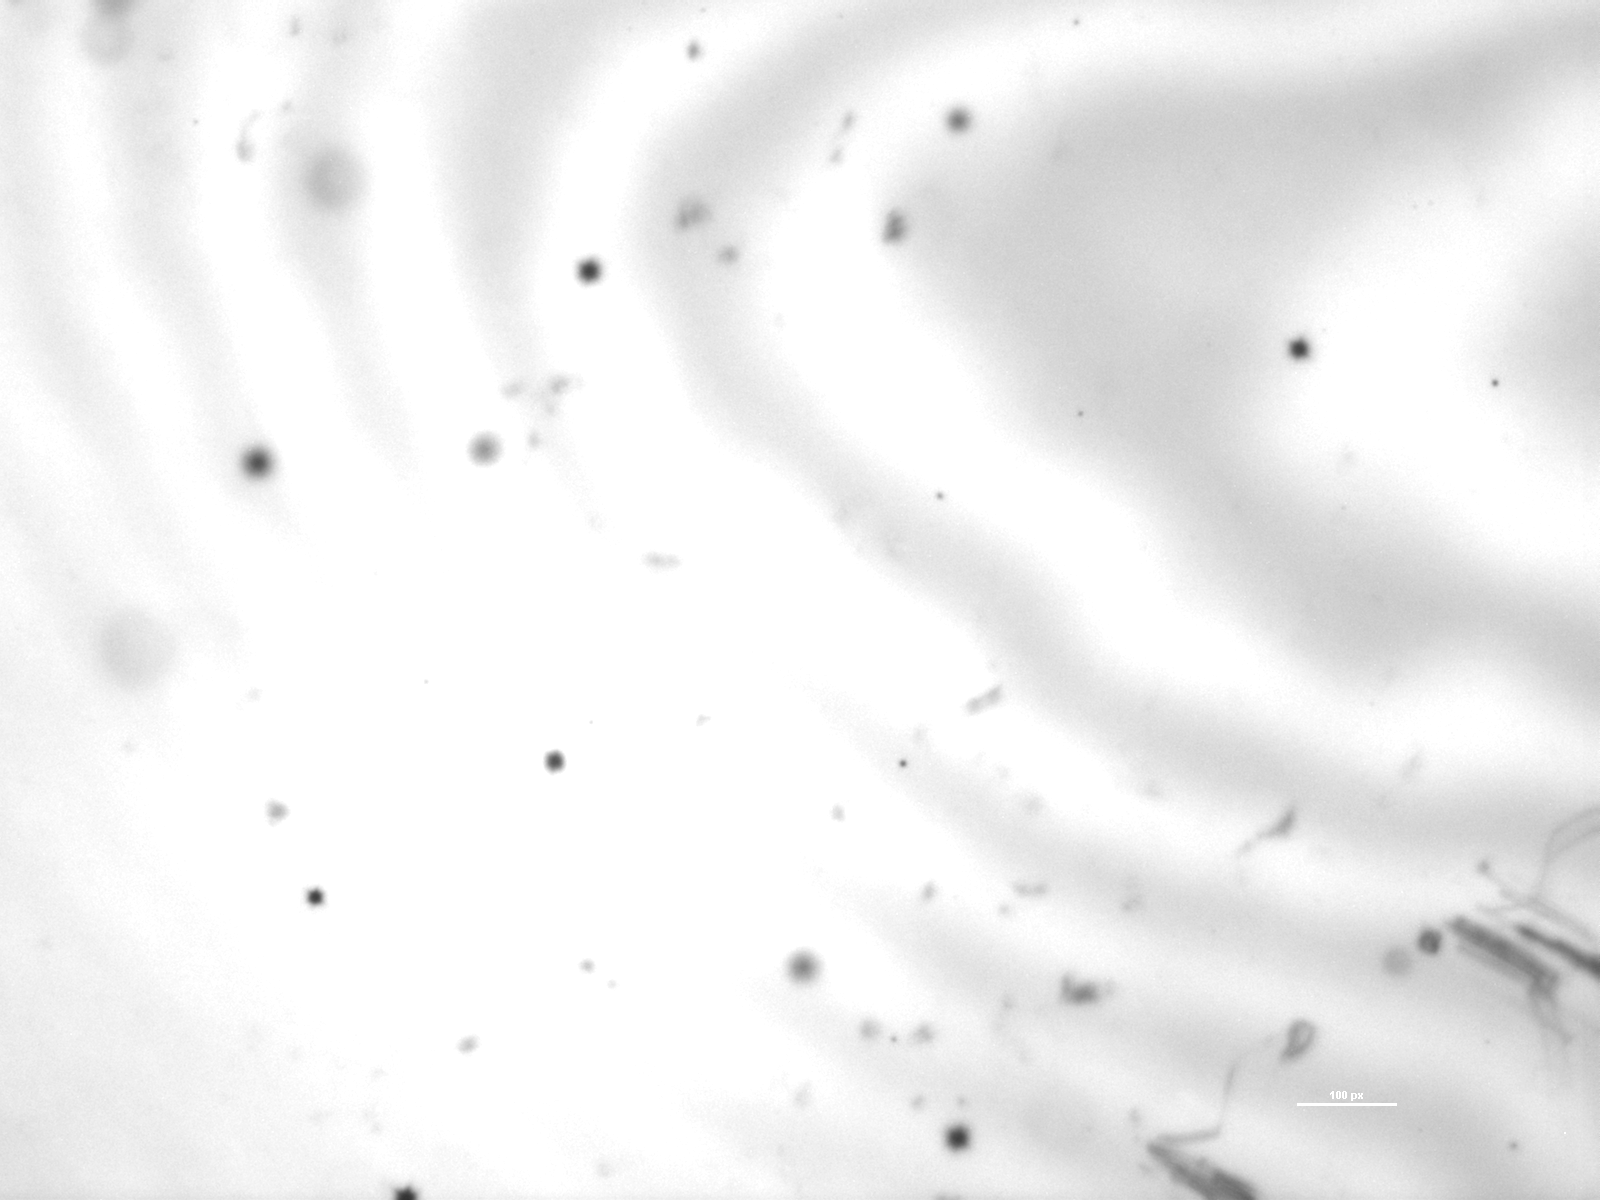
\includegraphics[scale=0.1]{obrazky/roztazeni_jasu_0_150.png}}
	\label{fig:jas_0_150}
	\caption{Přebarvení vysokých jasů s~mezní hodnotou 150 a roztažení}
	\end{figure}
	
	\begin{figure}[!htb]
	\centering
	\fbox{
\includegraphics[scale=0.1]{obrazky/roztazeni_jasu_0_125.png}}
	\label{fig:jas_0_125}
	\caption{Přebarvení vysokých jasů s~mezní hodnotou 125 a roztažení}
	\end{figure}				
		
	Segmentace snímku bude vzhledem k~množství dat řešena prahováním, které je výpočetně nejméně náročné. Metoda rozplavu je sice výpočetně srovnatelná, ale pro náš případ, kdy potřebujeme zvýraznit krajní hodnoty (0 až mez), \uv{degraduje} na metodu prahování. Hodnota prahu bude nastavena ručně uživatelem z~důvodu možného rozdílného rozložení hodnot jasu v~různých snímcích. V~testovací sekvenci snímků se jako vhodný práh jeví hodnota jasu mezi 160 a 190 (viz obrázky 3.7 a 3.8).
	
	\begin{figure}[!htb]
	\centering
	\fbox{
\includegraphics[scale=0.25]{obrazky/prahovani160_vyrez.png}}
	\label{fig:prahovani_160}
	\caption{Prahování s hodnotou prahu 160}
	\end{figure}
	
	\begin{figure}[!htb]
	\centering
	\fbox{
\includegraphics[scale=0.25]{obrazky/prahovani190_vyrez.png}}
	\label{fig:prahovani_190}
	\caption{Prahování s hodnotou prahu 190}
	\end{figure}
	
	\section{Detekce inkluzí}
V další fázi se budou detekovat inkluze.

\chapter{Popis implementace}
Volba programových prostředků: OpenCV verze 2.4 (hlavní verze, snadno dostupná na všech platformách, doporučení???)
	Cleaner - vtvoří šedotón, 

\chapter{Uživatelská dokumentace}
	\section{SW požadavky}
	
	\section{Adresářová struktura odevzdávaného souboru}	
	
	\section{Spuštění a ovládání aplikace}	

\chapter{Závěr}
Cílem této semestrální práce bylo vytvořit aplikaci pro detekci inkluzí.

\end{document} 
